\documentclass[12pt, a4paper, oneside]{article}\usepackage{graphicx, color}
%% maxwidth is the original width if it is less than linewidth
%% otherwise use linewidth (to make sure the graphics do not exceed the margin)
\makeatletter
\def\maxwidth{ %
  \ifdim\Gin@nat@width>\linewidth
    \linewidth
  \else
    \Gin@nat@width
  \fi
}
\makeatother

\definecolor{fgcolor}{rgb}{0.2, 0.2, 0.2}
\newcommand{\hlnumber}[1]{\textcolor[rgb]{0,0,0}{#1}}%
\newcommand{\hlfunctioncall}[1]{\textcolor[rgb]{0.501960784313725,0,0.329411764705882}{\textbf{#1}}}%
\newcommand{\hlstring}[1]{\textcolor[rgb]{0.6,0.6,1}{#1}}%
\newcommand{\hlkeyword}[1]{\textcolor[rgb]{0,0,0}{\textbf{#1}}}%
\newcommand{\hlargument}[1]{\textcolor[rgb]{0.690196078431373,0.250980392156863,0.0196078431372549}{#1}}%
\newcommand{\hlcomment}[1]{\textcolor[rgb]{0.180392156862745,0.6,0.341176470588235}{#1}}%
\newcommand{\hlroxygencomment}[1]{\textcolor[rgb]{0.43921568627451,0.47843137254902,0.701960784313725}{#1}}%
\newcommand{\hlformalargs}[1]{\textcolor[rgb]{0.690196078431373,0.250980392156863,0.0196078431372549}{#1}}%
\newcommand{\hleqformalargs}[1]{\textcolor[rgb]{0.690196078431373,0.250980392156863,0.0196078431372549}{#1}}%
\newcommand{\hlassignement}[1]{\textcolor[rgb]{0,0,0}{\textbf{#1}}}%
\newcommand{\hlpackage}[1]{\textcolor[rgb]{0.588235294117647,0.709803921568627,0.145098039215686}{#1}}%
\newcommand{\hlslot}[1]{\textit{#1}}%
\newcommand{\hlsymbol}[1]{\textcolor[rgb]{0,0,0}{#1}}%
\newcommand{\hlprompt}[1]{\textcolor[rgb]{0.2,0.2,0.2}{#1}}%

\usepackage{framed}
\makeatletter
\newenvironment{kframe}{%
 \def\at@end@of@kframe{}%
 \ifinner\ifhmode%
  \def\at@end@of@kframe{\end{minipage}}%
  \begin{minipage}{\columnwidth}%
 \fi\fi%
 \def\FrameCommand##1{\hskip\@totalleftmargin \hskip-\fboxsep
 \colorbox{shadecolor}{##1}\hskip-\fboxsep
     % There is no \\@totalrightmargin, so:
     \hskip-\linewidth \hskip-\@totalleftmargin \hskip\columnwidth}%
 \MakeFramed {\advance\hsize-\width
   \@totalleftmargin\z@ \linewidth\hsize
   \@setminipage}}%
 {\par\unskip\endMakeFramed%
 \at@end@of@kframe}
\makeatother

\definecolor{shadecolor}{rgb}{.97, .97, .97}
\definecolor{messagecolor}{rgb}{0, 0, 0}
\definecolor{warningcolor}{rgb}{1, 0, 1}
\definecolor{errorcolor}{rgb}{1, 0, 0}
\newenvironment{knitrout}{}{} % an empty environment to be redefined in TeX

\usepackage{alltt} % Paper size, default font size and one-sided paper
%\graphicspath{{./Figures/}} % Specifies the directory where pictures are stored
%\usepackage[dcucite]{harvard}
\usepackage{rotating}
\usepackage{amsmath}
\usepackage{setspace}
\usepackage{pdflscape}
\usepackage[flushleft]{threeparttable}
\usepackage{multirow}
\usepackage[comma, sort&compress]{natbib}% Use the natbib reference package - read up on this to edit the reference style; if you want text (e.g. Smith et al., 2012) for the in-text references (instead of numbers), remove 'numbers' 
\usepackage{graphicx}
%\bibliographystyle{plainnat}
\bibliographystyle{agsm}
\usepackage[colorlinks = true, citecolor = blue, linkcolor = blue]{hyperref}
%\hypersetup{urlcolor=blue, colorlinks=true} % Colors hyperlinks in blue - change to black if annoying
%\renewcommand[\harvardurl]{URL: \url}
 \usepackage{listings}
 \usepackage{color}
 \graphicspath{{../Pictures/}}
\definecolor{mygrey}{gray}{0.95}
\lstset{backgroundcolor=\color{mygrey}}
\IfFileExists{upquote.sty}{\usepackage{upquote}}{}
\begin{document}
\title{Using Thomson-Reuters Eikon}
\author{Rob Hayward}
%\date{\today}
\maketitle
%\begin{abstract}
%erehrere
%\end{abstract}
The Thomson-Reuters Eikon system provides real-time news and prices for financial securities as well as historical financial and economic data and some analytical tools.  The system can be used on any machine in Mithras Annex room 101.  To access the Annex after 5 o'clock in the evening, it is necessary to use the Unicard.  

You will need to access Thomson-Reuters from the applications folder.  You will be asked for a username and password.  We have five access points.  Four of these are currently operating from the Annex.  These are the usernames and passwords.  If someone is already using that username or password, you will be asked if you want to end their session. Please do not bump people out of their session. You should try another username and password.  If they are all being used, speak to the other people in Annex 101 and manage the access. 

If there are problems with the usernames and passwords, let me know 

rh49@brighton.ac.uk

\section*{Usernames and passwords}
These are the usernames and passwords. 

\hspace{6cm}

\begin{tabular}{l l l}
Number & Username & Password\\
\hline
1 & student2@ubbs.co.uk & Baifcms23\\
2 & student3@ubbs.co.uk & Pjy604123\\
3 & student4@ubbs.co.uk & Bacci46j? \\
4 & student5@ubbs.co.uk & Rdy26240\\
\end{tabular}

\section*{Navigation}
The system will open in whatever was last being viewed by the person using that username.  It is probably best to go back to the home page (called home).  This is a portal that will show the latest news and some market data and it will allow you to access all the other resources.  

There are generally two methods of getting around

Through asset class.  Across the left of the home screen, you will see the asset classes running from equities, through fixed income, FX and money markets and into commodities.  Therefore, if you are interested in corporate information, start with equities and drill down to what you want.  A very good way to get information about companies is to go to \emph{company view}.  This can be accessed from \emph{equities} and then  \emph{market data and tools}. 

You should see a page like this.  You can search for other companies using the \emph{search} function.  This is identified by a large magnifying glass. 

\begin{figure}[h!]
\centering
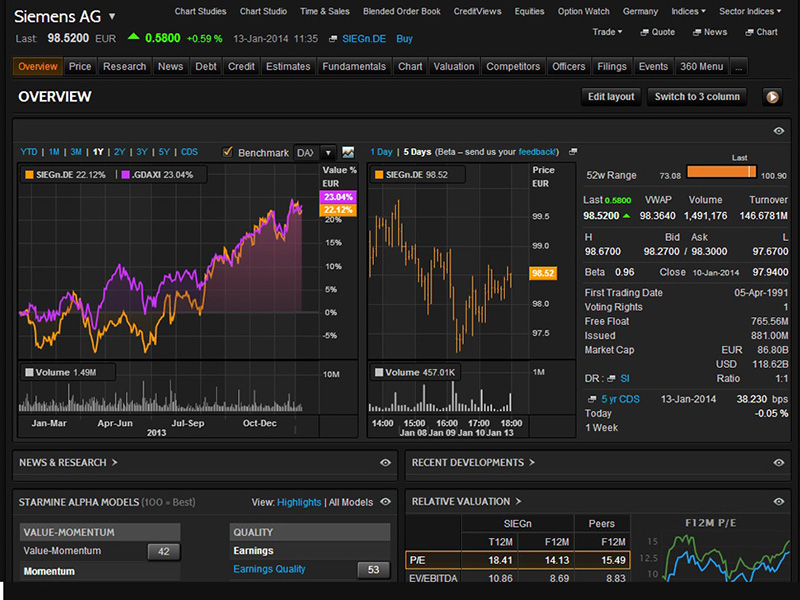
\includegraphics[scale = 0.6]{TR-Siemens}
\end{figure}

The other main avenue would be to search by country.  This can also be accessed from the home page.  There is a tab called \emph{country}.  This will take you to a country portal that will give access to news as well as economic and financial data.  The portal should look like this. 

\begin{figure}[h!]
\centering
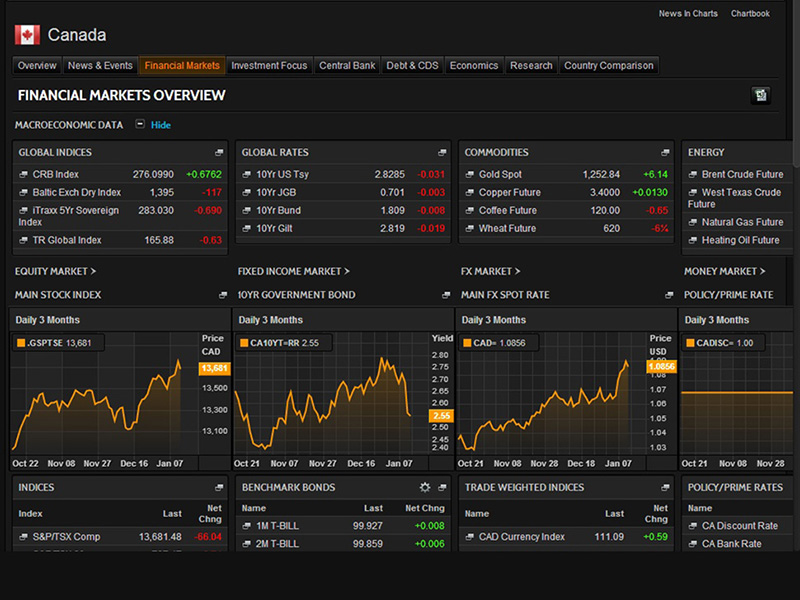
\includegraphics[scale = 0.6]{TR-Canada}
\end{figure}

There are also a number of financial models that can be used for calculating the value of securities or derivatives. These are usually accessed by the \emph{market data and tools} tab. 

\end{document}
